\section{Elektrotechnik}

\begin{defi}{Elektische Ladung}
    Grundlegende Eigenschaft von Materie: [Q] = C (Coulomb)

    Ladung ist beobachtbar als nicht mit Gravitation erklärbare Kraftwirkung zwischen Materie.

    Körper mit gleicher Ladung stoßen sich ab.
    Ungleich geladene Körper ziehen sich an.

    F ist definiert als Coulomb-Kraft:

    \[
        F = K \cdot \frac{Q_1 \cdot Q_2}{r^2} \cdot \vec{r}
    \]
\end{defi}

\begin{defi}{Arbeit}
    Potenzielle Energie: [W] = J (Joule)

    W ist proportional zur Größe der bewegten Ladung Q.
    Energie, die als Ergebnis einer Ladungsträgerverschiebung bezogen auf die Ladungseinheit zur Verfügung:

    \[
        U = \frac{W}{Q}
    \]
\end{defi}

\begin{defi}{Spannung}
    Spannung: [U] = V (Volt)

    \[
        V = \frac{J}{C}
    \]

    In der Regel gibt man die Spannung eines Punktes immer in Bezug auf einen festen Nullpunkt an.
\end{defi}

\begin{defi}{Stromstärke}
    Gerichtete Bewegung in Ladungsträgern: [I] = A (Ampere)

    \[
        I = \frac{\Delta Q}{\Delta t}
    \]
\end{defi}

\begin{defi}{Widerstand}
    Widerstand gegen Ausgleichsbewegungen freier Ladungsträger: [R] = $\Omega$ (Omega)

    \[
        R = \frac{U}{I} = \sum_{i = 1}^n R_i
    \]

    \begin{center}
        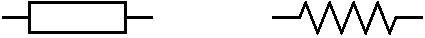
\includegraphics[width=0.35\textwidth]{includes/figures/widerstand.pdf}
    \end{center}
\end{defi}

\begin{defi}{Kirchhoffsche Regeln}
    \begin{itemize}
        \item \emph{Knotenregel}:

              Die Summe aller zufließenden Ströme in einem Punkt ist gleich der Summe der abfließenden Ströme.

              \[
                  \sum_{i \in \{1, \ldots, n\}} I_{\text{in}_i} - \sum_{i \in \{1, \ldots, n\}} I_{\text{out}_i} \stackrel{!}{=} 0
              \]
        \item \emph{Maschenregel}:

              Die Summer aller abfallenden Spannungen in einem Schaltkreis ist gleich Null.

              \[
                  - U_Q + \sum_{i \in \{1, \ldots, n\}} U_i \stackrel{!}{=} 0
              \]
        \item \emph{Anwendungen}:
        \item \emph{Maschenstromverfahren}:
    \end{itemize}
\end{defi}